\subsection{Half-Duplex Speech Interaction}
\label{sec:half-duplex}

Building on the preceding speech representations and components,
half-duplex systems organize perception and generation into
turn-based dialogue.
Within speech dialogue, core model modalities define three categories:
text-to-text in cascaded systems, speech-to-text in Thinker-Talker
systems, and speech-to-speech representation modeling in native
end-to-end systems.
This progression shifts text from mediating both input and output
to organizing replies after direct speech perception, then brings
speech representations into response generation.
It shapes how vocal cues inform reply content and spoken expression.
Incremental processing and streaming generation operate within
alternating turns.

\begin{figure}[htbp]
    \centering
    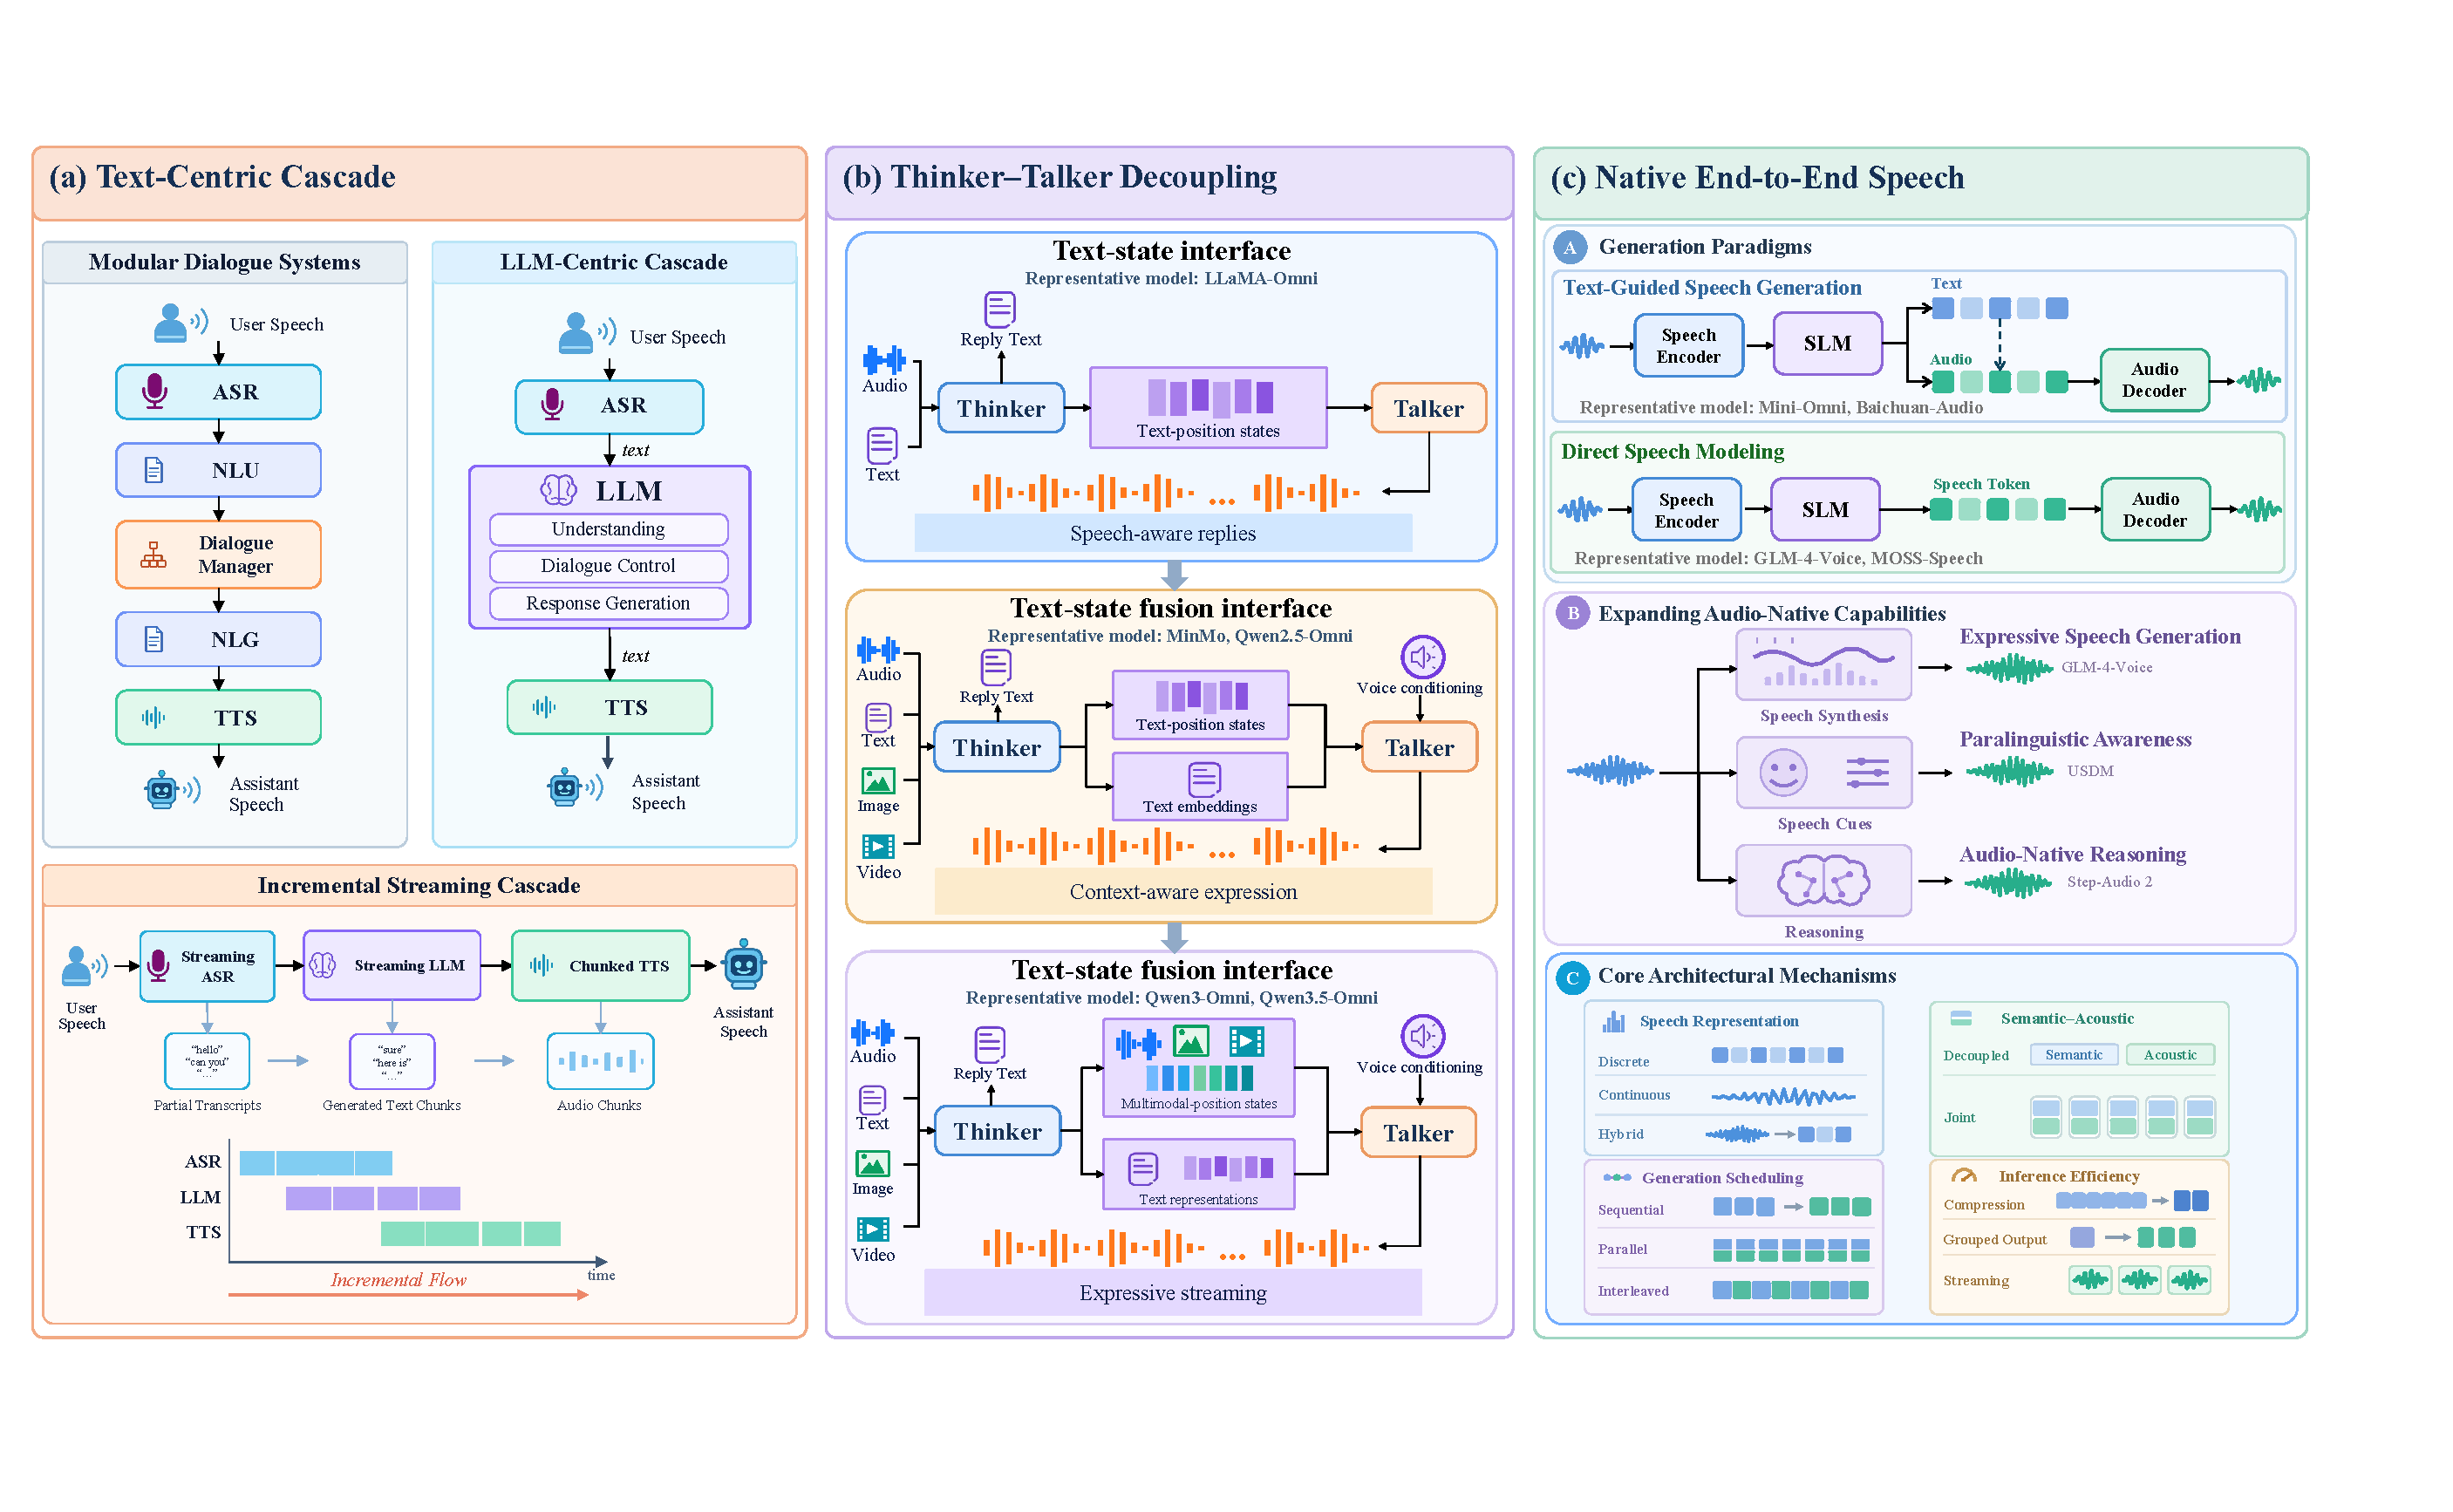
\includegraphics[width=\textwidth]{figures/half-duplex-overview.pdf}
    \caption{    
    Overview of half-duplex speech interaction architectures.
    (a) Text-centric cascaded interaction, comprising modular dialogue
    systems, LLM-centered cascades, and incremental streaming pipelines.
    (b) Thinker-Talker decoupled interaction with response-state
    conditioning (top), text-state fusion (middle), and multimodal-state
    sharing (bottom).
    (c) Native end-to-end speech interaction, comprising text-guided
    generation and direct speech modeling (top), audio-native capabilities
    (middle), and core architectural mechanisms (bottom).
    Streaming and overlapping computation operate within alternating
    conversational turns.
    }
    \label{fig:half-duplex-overview}
\end{figure}


\subsubsection{Text-Centric Cascaded Interaction}
\label{sec:text-centric-cascaded-interaction}

Text-centric cascaded interaction operates on the principle of mapping speech to textual counterparts for perception, reasoning, and generation. In this paradigm, text serves as the principal intermediary: recognition converts user speech into transcripts, from which the dialogue core interprets intentions, maintains context, and formulates a textual reply for synthesis~\citep{DBLP:journals/csur/McTear02,DBLP:journals/corr/abs-2411-13577}. Historically, the intermediate processing relied on highly fragmented pipelines, which have progressively evolved into more unified language backbones. The contemporary ASR $\rightarrow$ LLM $\rightarrow$ TTS architecture represents the current apex of this text-centric philosophy. In the half-duplex setting, users and systems alternate turns while internal processing can overlap. Figure~\ref{fig:half-duplex-overview}(a) traces this evolution,and Table~\ref{tab:half-duplex-systems} summarizes representative cascaded systems and related methods.

% % Required packages: booktabs, graphicx

\begin{table*}[t]
    \centering
    \caption{
        Text-centric cascaded systems and methods.
        \textit{Note.} SDS: spoken dialogue system.
        Interface identifies model-facing or inter-module representations;
        Execution highlights control and scheduling (``--'': outside scope).
        Text-only models provide language-side foundations;
        frameworks are compared through their cascaded paths.
        Streaming and internal overlap can operate within alternating turns.
    }
    \label{tab:text-centric-cascaded-comparison}
    \small
    \renewcommand{\arraystretch}{1.12}
    \setlength{\tabcolsep}{5pt}

    \resizebox{\textwidth}{!}{
    \begin{tabular}{l|l|l|l|l|l}
        \toprule
        \textbf{Work}
        & \textbf{Type}
        & \textbf{Interface}
        & \textbf{Language Core}
        & \textbf{Execution}
        & \textbf{Key Feature} \\
        \midrule

        \multicolumn{6}{l}{
            \textit{Modular systems and language-side consolidation}
        } \\
        \midrule

        GALAXY-II \citep{DBLP:conf/interspeech/SeneffHLPSZ98}
        & Architecture
        & Symbolic messages
        & Modular
        & Hub-controlled
        & Programmable distributed hub \\

        RavenClaw \citep{DBLP:journals/csl/BohusR09}
        & Framework
        & Symbolic representations
        & Modular
        & Task-driven
        & Task--skill separation \\

        POMDP SDS \citep{DBLP:journals/pieee/YoungGTW13}
        & Method
        & ASR/NLU hypotheses
        & Modular
        & Belief-driven
        & Uncertainty-aware control \\

        Wen et al. \citep{DBLP:conf/eacl/Rojas-BarahonaG17}
        & Model
        & Text
        & Neural TOD
        & --
        & Text-level end-to-end learning \\

        Sequicity \citep{DBLP:conf/acl/KanHLJRY18}
        & Model
        & Text
        & Seq2seq
        & --
        & Explicit belief span \\

        SimpleTOD \citep{DBLP:conf/nips/Hosseini-AslMWY20}
        & Model
        & Text
        & Causal LM
        & Autoregressive
        & State--action--response serialization \\

        SOLOIST \citep{DBLP:journals/tacl/PengLLSLG21}
        & Model
        & Text
        & Pretrained LM
        & Autoregressive
        & Transfer and machine teaching \\

        \midrule
        \multicolumn{6}{l}{
            \textit{Modern cascades and capability integration}
        } \\
        \midrule

        AudioGPT \citep{DBLP:conf/aaai/HuangLYSCYWHHLR24}
        & Agent
        & Text / tool calls
        & ChatGPT
        & Tool-orchestrated
        & External audio models \\

        ESPnet-SDS \citep{DBLP:conf/naacl/Arora0STCBFKTSS25}
        & Toolkit
        & Configurable
        & Configurable
        & Configurable
        & Cascade / E2E evaluation \\

        Eva \citep{DBLP:conf/ifaamas/QinZ25}
        & Agent
        & Text / tool calls
        & LLM
        & Agent-orchestrated
        & RAG, agents, telephony \\

        LiveKit Agents \citep{livekitagentsdocs}
        & Framework
        & Pipeline-dependent
        & Swappable
        & Configurable streaming
        & Pipeline / provider selection \\

        Pipecat \citep{pipecatdocs}
        & Framework
        & Frames
        & Swappable
        & Frame-streaming
        & Frame-based processors \\

        \midrule
        \multicolumn{6}{l}{
            \textit{Incremental processing and latency optimization}
        } \\
        \midrule

        Schlangen \& Skantze \citep{DBLP:journals/dad/SchlangenS11}
        & Method
        & Incremental units
        & Agnostic
        & Incremental
        & Revision and commitment \\

        InproTK \citep{DBLP:conf/naacl/BaumannS12}
        & Toolkit
        & Incremental units
        & Modular
        & Incremental
        & Reusable incremental modules \\

        Skantze \& Hjalmarsson \citep{DBLP:journals/csl/SkantzeH13}
        & Method
        & Incremental representations
        & Modular
        & Incremental
        & Planning and self-monitoring \\

        Telecom Agent \citep{DBLP:journals/corr/abs-2508-04721}
        & Agent
        & Text
        & 4-bit LLM
        & Concurrent
        & Domain ASR/TTS + RAG \\

        LTS-VoiceAgent \citep{DBLP:journals/corr/abs-2601-19952}
        & Agent
        & Partial text
        & LLM
        & Semantically triggered
        & \textit{When to think} \\

        DDTSR \citep{DBLP:journals/corr/abs-2602-23266}
        & Method
        & Streaming text
        & LLM
        & Cross-stage overlap
        & \textit{Speak while thinking} \\

        \bottomrule
    \end{tabular}
    }

\end{table*}


\paragraph{Textual representation and unified understanding.}
Textual representations support the interpretation of user utterances, the tracking of dialogue context, and the reasoning required for task execution. Classical systems distributed these responsibilities across distinct language understanding, dialogue management, and language generation modules~\citep{DBLP:journals/csur/McTear02}. POMDP-based managers maintained beliefs over uncertain recognition results and user intentions to guide dialogue decisions~\citep{DBLP:journals/pieee/YoungGTW13}. Neural models subsequently brought these functions into shared modeling: SimpleTOD, for instance, serialized belief states, dialogue actions, and responses within a single causal language model~\citep{DBLP:conf/nips/Hosseini-AslMWY20}. Modern LLM-centered systems further consolidate contextual interpretation, response generation, and tool orchestration, exemplified by AudioGPT's use of ChatGPT to coordinate external audio models~\citep{DBLP:conf/aaai/HuangLYSCYWHHLR24}. Consequently, while language-side processing has become highly unified, it continues to rely on text transcripts to represent the user's spoken input.

\paragraph{Response modeling and the text bottleneck.}
Reply formation connects the interpreted request and dialogue context to a response decision, its verbal formulation, and its spoken realization. While modular systems separate dialogue policy from language generation, shared autoregressive models now jointly generate dialogue actions and condition reply text on them~\citep{DBLP:journals/csur/McTear02,DBLP:conf/nips/Hosseini-AslMWY20}. The resulting text carries the lexical content to the TTS module. However, relying solely on text creates an inherent bottleneck with two major gaps: input transcripts incompletely preserve vocal cues (e.g., emotion, intonation) relevant to deciding \textit{how} to respond, and output text underspecifies the intended prosody and speaking style for synthesis~\citep{DBLP:conf/acl/CuiYJMZWGK25}. FireRedChat illustrates the input boundary through its text-only cascaded LLM and its audio-aware semi-cascaded alternative~\citep{chen2025fireredchat}. Auxiliary descriptions can partly bridge these gaps; for example, X-Talk injects acoustic descriptions into the LLM's system prompt and allows the adjustment of TTS emotion vectors~\citep{DBLP:journals/corr/abs-2512-18706}. Nevertheless, their coverage remains bounded by what analysis modules can extract and synthesis controls can express, meaning text-mediated coordination inherently limits the preservation of rich acoustic information.

\paragraph{Component optimization and interface coordination.}
Explicit textual interfaces allow recognition, dialogue processing, and synthesis to be trained, evaluated, adapted, or replaced independently. ESPnet-SDS supports configurable pipelines and rigorous component evaluation~\citep{DBLP:conf/naacl/Arora0STCBFKTSS25}; Eva integrates telephony, retrieval, and task agents around a speech dialogue pipeline~\citep{DBLP:conf/ifaamas/QinZ25}; and LiveKit Agents exposes interchangeable speech and language providers for developers~\citep{livekitagentsdocs}. Such modularity supports extensive reuse and application-specific adaptation, but it requires connected components to exchange compatible information. Coordination can also be learned locally to smooth the interfaces: DDTSR trains a lightweight connective model to ensure continuity with subsequent large-model replies, progressively adapting it to partial inputs~\citep{DBLP:journals/corr/abs-2602-23266}. Independent component improvements therefore necessitate interface-level checks, as recognition errors can cascade to alter downstream decisions, and a semantically correct reply still requires suitable formatting for its intended vocal delivery.

\paragraph{Streaming execution and output commitment.}
Waiting for complete transcripts and full LLM replies creates latency barriers between perception, response formation, and synthesis. Incremental execution addresses this by letting downstream stages process partial results. Schlangen and Skantze formalized this through revisable and committed hypotheses~\citep{DBLP:journals/dad/SchlangenS11}, while frameworks like Pipecat implement streaming orchestration via frame processors~\citep{pipecatdocs}. Scheduling mechanisms must decide when to trigger reasoning and when to synthesize available text. LTS-VoiceAgent triggers reasoning from informative speech prefixes~\citep{DBLP:journals/corr/abs-2601-19952}, and DDTSR prepares short connectives from partial transcripts while a larger model computes the substantive reply~\citep{DBLP:journals/corr/abs-2602-23266}. However, earlier execution introduces revision costs: changing transcripts can invalidate speculative replies, and already-played speech requires conversational repair. Hypothesis revision, cancellation, and output commitment therefore govern the delicate balance between responsiveness and stability~\citep{DBLP:journals/dad/SchlangenS11}. Consequently, evaluation must distinguish \textit{time to first audio} from \textit{time to substantive response}, as early connectives can advance the onset without delivering the actual answer~\citep{DBLP:journals/corr/abs-2602-23266}. 

Ultimately, while incremental execution mitigates latency, cascaded systems remain constrained by their text-centric architecture. Relying on transcripts loses rich vocal cues, risks cascading errors, and forces complex trade-offs between responsiveness and revision costs. To bypass this text bottleneck, Thinker-Talker systems evolve the paradigm by bringing continuous speech representations directly into the understanding backbone.

\subsubsection{Thinker-Talker Decoupled Interaction}
\label{sec:thinker-talker-decoupled-interaction}
Thinker-Talker interaction centers on an audio understanding model that directly receives continuous speech representations and formulates its response as text. The Thinker retains language capabilities for semantic understanding and deep reasoning over audio and dialogue history, while the Talker can use its hidden states and text conditions for streaming speech after turn handover~\citep{DBLP:journals/corr/abs-2501-06282,DBLP:journals/corr/abs-2503-20215,DBLP:journals/corr/abs-2509-17765}. Their decoupled optimization combines understanding depth with generation efficiency~\citep{DBLP:conf/icml/WangLFZS000M25}. This paradigm has become a mainstream approach to optimizing end-to-end half-duplex speech interaction~\citep{DBLP:conf/iclr/FangGZMZ025,DBLP:journals/corr/abs-2501-06282,DBLP:journals/corr/abs-2503-20215,DBLP:journals/corr/abs-2509-17765}. Figure~\ref{fig:half-duplex-overview}(b) illustrates the evolution
of Thinker-Talker information sharing, and
Table~\ref{tab:half-duplex-systems} summarizes representative
systems and their architectural highlights.

\paragraph{Continuous speech representations for language understanding.}
The Thinker's input interface aligns continuous audio encoder features
with a pretrained language backbone to support speech understanding
and text response formulation~\citep{DBLP:conf/iclr/FangGZMZ025,DBLP:journals/corr/abs-2501-06282,DBLP:journals/corr/abs-2503-20215}.
LLaMA-Omni uses a speech adapter~\citep{DBLP:conf/iclr/FangGZMZ025},
while MinMo employs input alignment to convey speech content,
emotion, and audio events~\citep{DBLP:journals/corr/abs-2501-06282}.
Uni-MoE combines audio and speech connectors with modality-specific
experts and progressive training for multimodal
understanding~\citep{DBLP:journals/pami/LiJHWZLMZ25}.
This alignment must preserve vocal cues and environmental sounds
that transcripts may lose so that they can inform language understanding,
reasoning, and response formulation.
When supported, incremental encoding begins as speech arrives;
in the half-duplex setting, spoken replies follow turn handover.

\paragraph{Hidden-state and text conditioning for speech generation.}
As the Thinker formulates a response, the interface must convey its lexical content to the Talker while retaining information relevant to spoken delivery. These interfaces differ in whether lexical content is carried
implicitly by internal representations or supplied explicitly as text,
with representative conditioning mechanisms summarized in
Table~\ref{tab:half-duplex-systems}.
LLaMA-Omni carries lexical content implicitly through response
hidden states~\citep{DBLP:conf/iclr/FangGZMZ025}, while other designs combine
text tokens or embeddings with internal representations through
prefix conditioning, projection, or fusion~\citep{DBLP:conf/icml/WangLFZS000M25,DBLP:journals/corr/abs-2501-06282,DBLP:journals/corr/abs-2503-20215,DBLP:journals/corr/abs-2505-02625}.
Beyond lexical content, shared representations allow user audio and
dialogue history to guide spoken delivery, while explicit voice
conditions provide additional control.
MinMo and Qwen2.5-Omni share user-query and dialogue-history
information~\citep{DBLP:journals/corr/abs-2501-06282,DBLP:journals/corr/abs-2503-20215}, while Qwen3-Omni
and Qwen3.5-Omni supply multimodal Thinker representations with
historical and streaming text; the latter also provides voice
conditions~\citep{DBLP:journals/corr/abs-2509-17765,DBLP:journals/corr/abs-2604-15804}.
Uni-MoE-2.0-Omni uses explicit conditioning, conveying response text and voice-control
prompts to a separate context-aware MoE-TTS
module~\citep{DBLP:journals/corr/abs-2511-12609}.
Effective transfer of these conditions helps the Talker
preserve response wording and adapt emphasis and affect to the
dialogue context, supporting consistency between semantic content
and acoustic expression.

% \begin{table}[t]
    \centering
    \caption{Thinker-Talker systems in turn-based speech dialogue: continuous audio inputs and text replies. Visual encoders indicate additional capabilities. AR/NAR: autoregressive/non-autoregressive; CTC: connectionist temporal classification; KV: key/value; MTP: multi-token prediction; AuT: Audio Transformer; TMRoPE: time-aligned multimodal rotary position embedding; ARIA: Adaptive Rate Interleave Alignment.}
    \label{tab:thinker-talker}
    \small
    \setlength{\tabcolsep}{4pt}
    \renewcommand{\arraystretch}{1.1}
    \begin{tabular}{@{}>{\raggedright\arraybackslash}p{\dimexpr0.18\linewidth-6pt\relax}>{\raggedright\arraybackslash}p{\dimexpr0.26\linewidth-6pt\relax}>{\raggedright\arraybackslash}p{\dimexpr0.29\linewidth-6pt\relax}>{\raggedright\arraybackslash}p{\dimexpr0.27\linewidth-6pt\relax}@{}}
        \toprule
        \textbf{System} & \textbf{Thinker}\newline Input / understanding & \textbf{Interface}\newline Talker conditions & \textbf{Talker}\newline Generation / streaming \\
        \midrule
        LLaMA-Omni\newline\citep{DBLP:conf/iclr/FangGZMZ025} & Whisper + adapter;\newline speech instructions & Response hidden states;\newline no separate text input & NAR/CTC units;\newline chunked vocoding \\
        \addlinespace
        Freeze-Omni\newline\citep{DBLP:conf/icml/WangLFZS000M25} & Streaming encoder + adapter; frozen LLM & Text tokens +\newline hidden-state prefix KV & NAR prefill + AR tokens;\newline streaming codec \\
        \addlinespace
        MinMo\newline\citep{DBLP:journals/corr/abs-2501-06282} & SenseVoice + projector;\newline speech, emotion, events & Text embeddings + query/response states; projection & AR tokens; fixed interleaving;\newline chunked flow matching \\
        \addlinespace
        Qwen2.5-Omni\newline\citep{DBLP:journals/corr/abs-2503-20215} & Audio/vision encoders;\newline TMRoPE alignment & Text embeddings + Thinker states; shared history & Dual-track AR;\newline sliding-window flow matching \\
        \addlinespace
        LLaMA-Omni~2\newline\citep{DBLP:journals/corr/abs-2505-02625} & Whisper + adapter;\newline multi-turn adaptation & Text embeddings + response states; gated fusion & AR read/write scheduling;\newline causal flow matching \\
        \addlinespace
        Qwen3-Omni\newline\citep{DBLP:journals/corr/abs-2509-17765} & AuT + vision encoder;\newline temporal-ID alignment & Historical/streaming text + multimodal states & AR + residual-codebook MTP;\newline causal ConvNet \\
        \addlinespace
        \mbox{Uni-MoE-2.0-Omni}\newline\citep{DBLP:journals/corr/abs-2511-12609}
        & Whisper/Q-Former + vision encoder;\newline 3D RoPE alignment
        & Text tokens + voice-control prompts
        & AR tokens; sentence-level streaming;\newline WavTokenizer decoding \\
        \addlinespace
        Qwen3.5-Omni\newline\citep{DBLP:journals/corr/abs-2604-15804} & AuT + vision encoder;\newline explicit timestamps & Historical/streaming text + multimodal states; voice prompt & ARIA interleaving;\newline multi-codebook prediction;\newline causal ConvNet \\
        \bottomrule
    \end{tabular}
\end{table}


\paragraph{Decoupled training and cross-module alignment.}
Decoupled training coordinates language and acoustic objectives while retaining the Thinker's language capabilities. On the understanding side, adaptation strategies differ in which components receive updates: the language backbone can remain frozen, as in Freeze-Omni, or be updated with the input adapter while the speech encoder stays frozen, as in LLaMA-Omni and LLaMA-Omni~2~\citep{DBLP:conf/icml/WangLFZS000M25,DBLP:conf/iclr/FangGZMZ025,DBLP:journals/corr/abs-2505-02625}. MinMo combines progressive input alignment with low-rank adaptation (LoRA) of the LLM, while the Qwen series unfreezes the language backbone during staged multimodal pretraining~\citep{DBLP:journals/corr/abs-2501-06282,DBLP:journals/corr/abs-2503-20215,DBLP:journals/corr/abs-2509-17765,DBLP:journals/corr/abs-2604-15804}. On the generation side, training aligns the interface and speech generator with the resulting representations. With the understanding side frozen, updates can be confined to a speech decoder or an added prefix decoder, as in LLaMA-Omni and Freeze-Omni, respectively~\citep{DBLP:conf/iclr/FangGZMZ025,DBLP:conf/icml/WangLFZS000M25}. Local joint optimization couples the interface with speech prediction: LLaMA-Omni~2 and MinMo jointly train their respective gate fusion module and output projector with the speech generation model~\citep{DBLP:journals/corr/abs-2505-02625,DBLP:journals/corr/abs-2501-06282}. Across both modules, the Qwen series uses specialized post-training for instruction following and reasoning in the Thinker, and contextual generation, preference alignment, and speaker control in the Talker~\citep{DBLP:journals/corr/abs-2503-20215,DBLP:journals/corr/abs-2509-17765,DBLP:journals/corr/abs-2604-15804}. These schedules aim to preserve response quality while aligning spoken content and expression with the intended answer.

\paragraph{Incremental speech prediction and streaming synthesis.}
After turn handover, timely and fluent spoken replies require coordination between text-derived conditions, speech-unit prediction, and waveform synthesis. Waiting for more text supplies context for pronunciation and prosody, while smaller increments support earlier playback. Incremental prediction and interleaved scheduling address this trade-off, with representative mechanisms summarized in Table~\ref{tab:half-duplex-systems}. Speech units can be emitted from incoming response hidden states using non-autoregressive prediction, as in LLaMA-Omni's decoder trained with connectionist temporal classification (CTC)~\citep{DBLP:conf/iclr/FangGZMZ025}. Autoregressive generation can instead interleave the consumption of text-derived conditions with speech prediction, as in MinMo~\citep{DBLP:journals/corr/abs-2501-06282}. Coordinating the different text and speech token rates is a further scheduling concern, addressed by Qwen3.5-Omni's Adaptive Rate Interleave Alignment (ARIA)~\citep{DBLP:journals/corr/abs-2604-15804}. Waveform synthesis then converts predicted units into playable segments through chunk-aware flow matching, as in CosyVoice~2 used by MinMo~\citep{DBLP:journals/corr/abs-2412-10117}, or causal convolutional decoding, as in Qwen3-Omni~\citep{DBLP:journals/corr/abs-2509-17765}. Together, incremental prediction and streaming synthesis shape how soon users hear the reply and how smoothly it continues, with generation scheduling governing the availability of speech units and synthesis throughput and chunk transitions affecting playback continuity.

Overall, Thinker-Talker interaction uses direct speech understanding and hidden-state sharing to make replies more contextually appropriate and spoken expression better aligned with intent. These gains depend on cross-module alignment and coordinated streaming for consistent, fluent delivery. While the Thinker organizes replies as text, native end-to-end interaction brings speech representations into both the input and output modeling of the dialogue backbone.


% Required packages: booktabs, array, tabularx

\begin{table*}[!tp]
    \centering
    \caption{
        Representative systems and methods for half-duplex speech interaction.
        SDS: spoken dialogue system; TOD: task-oriented dialogue;
        CTC: connectionist temporal classification;
        ARIA: Adaptive Rate Interleave Alignment.
        FireRedChat is shown in its cascaded configuration.
    }
    \label{tab:half-duplex-systems}
    \scriptsize
    \setlength{\tabcolsep}{3pt}
    \renewcommand{\arraystretch}{1.3}

    \begin{tabularx}{\textwidth}{
        @{}
        >{\raggedright\arraybackslash}p{0.25\textwidth}
        >{\raggedright\arraybackslash}p{0.13\textwidth}
        >{\raggedright\arraybackslash}p{0.24\textwidth}
        >{\raggedright\arraybackslash}X
        @{}
    }
        \toprule
        \textbf{System / Work}
        & \textbf{Architecture}
        & \textbf{Input / Output}
        & \textbf{Highlight} \\
        \midrule

        \multicolumn{4}{@{}l}{\textit{Text-centric cascaded systems and methods}} \\
        \midrule

        GALAXY-II~\citep{DBLP:conf/interspeech/SeneffHLPSZ98}
        & Modular SDS & Speech / Speech
        & Programmable hub for distributed modules \\

        POMDP SDS~\citep{DBLP:journals/pieee/YoungGTW13}
        & Modular SDS & Speech / Speech
        & Belief-state dialogue control \\

        SimpleTOD~\citep{DBLP:conf/nips/Hosseini-AslMWY20}
        & Text-only TOD & Text / Text
        & State--action--response serialization \\

        AudioGPT~\citep{DBLP:conf/aaai/HuangLYSCYWHHLR24}
        & Cascade & Text, Audio, Image, Score / Text, Audio, Video
        & LLM orchestration of audio tools \\

        ESPnet-SDS~\citep{DBLP:conf/naacl/Arora0STCBFKTSS25}
        & Configurable & Configurable
        & Cascade and end-to-end evaluation \\

        Eva~\citep{DBLP:conf/ifaamas/QinZ25}
        & Cascade & Speech / Speech
        & Retrieval and telephony integration \\

        LiveKit Agents~\citep{livekitagentsdocs}
        & Configurable & Pipeline-dependent
        & Interchangeable speech and language providers \\

        Pipecat~\citep{pipecatdocs}
        & Configurable & Pipeline-dependent
        & Frame-based streaming processors \\

        Schlangen \& Skantze~\citep{DBLP:journals/dad/SchlangenS11}
        & Modular & Modality-agnostic
        & Incremental units with revision and commitment \\

        InproTK~\citep{DBLP:conf/naacl/BaumannS12}
        & Modular & Configurable
        & Reusable incremental processing modules \\

        Telecom Agent~\citep{DBLP:journals/corr/abs-2508-04721}
        & Cascade & Speech / Speech
        & Domain ASR/TTS; concurrent execution \\

        FireRedChat~\citep{DBLP:journals/corr/abs-2509-06502}
        & Cascade & Speech / Text, Speech
        & Pluggable cascade; streaming synthesis \\

        LTS-VoiceAgent~\citep{DBLP:journals/corr/abs-2601-19952}
        & Cascade & Speech / Text
        & Speech-prefix triggers for reasoning \\

        DDTSR~\citep{DBLP:journals/corr/abs-2602-23266}
        & Cascade & Speech / Speech
        & Early connectives; cross-stage overlap \\

        \midrule
        \multicolumn{4}{@{}l}{\textit{Thinker-Talker decoupled systems}} \\
        \midrule

        LLaMA-Omni~\citep{DBLP:conf/iclr/FangGZMZ025}
        & Thinker-Talker & Speech / Text, Speech
        & Response states; CTC decoding \\

        Freeze-Omni~\citep{DBLP:conf/icml/WangLFZS000M25}
        & Thinker-Talker & Text, Speech / Text, Speech
        & Frozen LLM; hidden-state prefix \\

        MinMo~\citep{DBLP:journals/corr/abs-2501-06282}
        & Thinker-Talker & Text, Audio / Text, Speech
        & Text and context states; interleaving \\

        Qwen2.5-Omni~\citep{DBLP:journals/corr/abs-2503-20215}
        & Thinker-Talker & Text, Audio, Image, Video / Text, Speech
        & Shared Thinker states; dual-track decoding \\

        LLaMA-Omni~2~\citep{DBLP:journals/corr/abs-2505-02625}
        & Thinker-Talker & Speech / Text, Speech
        & Gated fusion; read/write scheduling \\

        Qwen3-Omni~\citep{DBLP:journals/corr/abs-2509-17765}
        & Thinker-Talker & Text, Audio, Image, Video / Text, Speech
        & Multimodal states; causal decoding \\

        Uni-MoE-2.0-Omni~\citep{DBLP:journals/corr/abs-2511-12609}
        & Thinker-Talker & Text, Audio, Image, Video / Text, Speech, Image
        & Text and voice prompts for MoE-TTS \\

        Qwen3.5-Omni~\citep{DBLP:journals/corr/abs-2604-15804}
        & Thinker-Talker & Text, Audio, Image, Video / Text, Speech
        & Multimodal and voice conditions; ARIA \\

        \midrule
        \multicolumn{4}{@{}l}{\textit{Native end-to-end speech systems}} \\
        \midrule

        SpeechGPT~\citep{DBLP:conf/emnlp/ZhangLZZWZQ23}
        & Native Speech & Text, Speech / Text, Speech
        & Discrete units; cross-modal tuning \\

        USDM~\citep{DBLP:conf/nips/KimSJKKKLSOHYY24}
        & Native Speech & Text, Speech / Text, Speech
        & Speech-text pretraining; prosody cues \\

        Mini-Omni~\citep{DBLP:journals/corr/abs-2408-16725}
        & Native Speech & Text, Speech / Text, Speech
        & Parallel text and audio generation \\

        IntrinsicVoice~\citep{DBLP:journals/corr/abs-2410-08035}
        & Native Speech & Text, Speech / Text, Speech
        & GroupFormer speech compression \\

        GLM-4-Voice~\citep{DBLP:journals/corr/abs-2412-02612}
        & Native Speech & Text, Speech / Text, Speech
        & Low-rate tokens; streaming decoding \\

        Flow-Omni~\citep{DBLP:journals/corr/abs-2412-04917}
        & Native Speech & Text, Speech / Text, Speech
        & Continuous speech via flow matching \\

        SLAM-Omni~\citep{DBLP:conf/acl/Chen0YLLXN00L0025}
        & Native Speech & Speech / Text, Speech
        & Grouped semantic tokens; vocoder \\

        Baichuan-Audio~\citep{DBLP:journals/corr/abs-2502-17239}
        & Native Speech & Text, Audio / Text, Speech
        & Joint semantic-acoustic codebooks \\

        Kimi-Audio~\citep{DBLP:journals/corr/abs-2504-18425}
        & Native Speech & Text, Audio / Text, Speech
        & Continuous inputs; discrete outputs \\

        VITA-Audio~\citep{DBLP:journals/corr/abs-2505-03739}
        & Native Speech & Text, Speech / Text, Speech
        & Multi-token audio prediction \\

        Step-Audio~2~\citep{DBLP:journals/corr/abs-2507-16632}
        & Native Speech & Text, Audio / Text, Speech
        & Audio-native reasoning with RL \\

        MOSS-Speech~\citep{DBLP:conf/iclr/ZhaoXJWCJCLCWZC26}
        & Native Speech & Speech / Speech
        & Modality-specific layers; no text guidance \\

        GPT-Realtime-2.1~\citep{openai2026gptrealtime21}
        & Native Speech & Text, Audio, Image / Text, Speech
        & Speech reasoning and tool calling \\

        Qwen-Audio~3.1+~\citep{alibaba2026qwenaudio31realtime}
        & Native Speech & Text, Audio / Text, Speech
        & Push-to-talk with function calling \\

        EVI~3~\citep{cowen2025evi3}
        & Native Speech & Text, Speech / Text, Speech
        & Coordinated content and prosody \\

        \bottomrule
    \end{tabularx}
\end{table*}

\subsubsection{Native End-to-End Speech Interaction}
\label{sec:native-end-to-end-speech-interaction}
Native end-to-end speech interaction uses a dialogue backbone that models speech representations on both the input and output paths: a speech language model sits between a speech encoder or tokenizer and a speech decoder, so that a turn proceeds as speech $\rightarrow$ speech representation $\rightarrow$ speech language model $\rightarrow$ speech representation $\rightarrow$ speech. Semantic content, prosody, emotion, and speaker characteristics can then inform the reply to the extent that the representations retain them. In the half-duplex setting, input may be encoded incrementally and response speech streams after turn handover; continuous listening and interruption during system speech belong to full-duplex interaction. Figure~\ref{fig:half-duplex-overview}(c) summarizes generation paradigms (A), audio-native capabilities (B), and core architectural mechanisms (C).

\paragraph{Discrete, continuous, and hybrid speech representations in the backbone.}
The paradigm originates in speech language modeling: GSLM modeled discrete self-supervised units with language-model objectives~\citep{lakhotia2021gslm}, and SpeechGPT brought such units into a pretrained text LLM that both receives and emits speech~\citep{DBLP:conf/emnlp/ZhangLZZWZQ23}. Representations first differ in form. Discrete tokens let speech reuse next-token prediction, as in GLM-4-Voice's low-rate single-codebook tokens~\citep{DBLP:journals/corr/abs-2412-02612}; Flow-Omni models continuous speech features alongside discrete text and generates speech through flow matching~\citep{DBLP:journals/corr/abs-2412-04917}; and Kimi-Audio pairs continuous inputs for understanding with discrete outputs for generation~\citep{DBLP:journals/corr/abs-2504-18425}. They also differ in whether semantic and acoustic information are decoupled or modeled jointly: SLAM-Omni predicts compact semantic tokens and leaves timbre and acoustic realization to the vocoder~\citep{DBLP:conf/acl/Chen0YLLXN00L0025}, whereas Baichuan-Audio keeps both in a multi-codebook representation~\citep{DBLP:journals/corr/abs-2502-17239}. Continuous or hybrid inputs retain more vocal cues for understanding, while discrete outputs keep generation within token prediction; decoupling shortens backbone sequences and eases alignment with text but leaves expressive detail to the decoder, whereas joint modeling keeps that detail in the backbone at the cost of longer sequences.

\paragraph{Text-guided generation, direct speech modeling, and vocal cues in response planning.}
The two generation paradigms differ in whether intermediate text guides what the reply says. Text-guided generation conditions audio on text from the same backbone, whether the text precedes speech units, as in SpeechGPT and USDM~\citep{DBLP:conf/emnlp/ZhangLZZWZQ23,DBLP:conf/nips/KimSJKKKLSOHYY24}, serves as a semantic channel that instructs audio generation, as in Mini-Omni~\citep{DBLP:journals/corr/abs-2408-16725}, or is interleaved with audio tokens to anchor content, as in Baichuan-Audio~\citep{DBLP:journals/corr/abs-2502-17239}. Direct speech modeling instead has the backbone predict speech tokens as its own output, as in GLM-4-Voice~\citep{DBLP:journals/corr/abs-2412-02612}; IntrinsicVoice reduces reliance on explicit text generation~\citep{DBLP:journals/corr/abs-2410-08035}, and MOSS-Speech removes text guidance through modality-based layer splitting~\citep{DBLP:conf/iclr/ZhaoXJWCJCLCWZC26}. Beyond content, native modeling moves vocal cues from rendering into planning: GLM-4-Voice shapes output prosody and style, USDM lets input prosody inform the reply, and Step-Audio~2's audio-native reasoning lets speaking style and emotion inform response behavior as well as voice~\citep{DBLP:journals/corr/abs-2507-16632}. Production systems combine these capabilities with reasoning and tool calling in GPT Realtime~2.1~\citep{openai2026gptrealtime21}, coordinated content and prosody in EVI~3~\citep{cowen2025evi3}, and function calling alongside a turn-based push-to-talk path in Qwen Audio~3.1 Realtime Plus~\citep{alibaba2026qwenaudio31realtime}. Text guidance stabilizes content through the backbone's language ability but limits expression to what text carries; direct modeling frees expression at the risk of weaker content control.

\paragraph{Unified pretraining, instruction tuning, freezing strategies, and reinforcement learning.}
Optimization must add speech modeling while retaining language capability; systems differ in which components are updated. SpeechGPT established modality-adaptation pretraining followed by cross-modal and chain-of-modality instruction tuning~\citep{DBLP:conf/emnlp/ZhangLZZWZQ23}. Later systems scale pretraining: USDM pretrains on unified speech-text sequences~\citep{DBLP:conf/nips/KimSJKKKLSOHYY24}, GLM-4-Voice and Baichuan-Audio pretrain on large-scale interleaved speech-text data before dialogue fine-tuning~\citep{DBLP:journals/corr/abs-2412-02612,DBLP:journals/corr/abs-2502-17239}, and Kimi-Audio pretrains jointly on audio and text before supervised fine-tuning~\citep{DBLP:journals/corr/abs-2504-18425}. Freezing strategies protect language ability at lower cost, as when Mini-Omni freezes the language model while aligning audio adapters~\citep{DBLP:journals/corr/abs-2408-16725} and MOSS-Speech trains added speech layers with the text layers frozen~\citep{DBLP:conf/iclr/ZhaoXJWCJCLCWZC26}. Reinforcement learning then shapes behavior beyond likelihood objectives, as in Step-Audio~2~\citep{DBLP:journals/corr/abs-2507-16632}. Interleaved pretraining aligns the modalities deeply but is expensive; freezing preserves text capability at the risk of weaker speech-text coordination, on which semantic-acoustic consistency depends.

\paragraph{Sequence compression, multi-token prediction, and streaming decoding.}
Speech sequences are far longer than text, so execution mechanisms govern startup latency and playback continuity. Compression shortens the sequence, through low-rate tokenization in GLM-4-Voice or GroupFormer's text-comparable lengths in IntrinsicVoice~\citep{DBLP:journals/corr/abs-2412-02612,DBLP:journals/corr/abs-2410-08035}, and grouped output reduces decoding steps, as SLAM-Omni predicts a group of semantic tokens per step~\citep{DBLP:conf/acl/Chen0YLLXN00L0025} and VITA-Audio's Multiple Cross-modal Token Prediction emits several audio tokens per forward pass~\citep{DBLP:journals/corr/abs-2505-03739}. Scheduling, independently of text guidance, determines when speech can begin: SpeechGPT and USDM complete the text first, Mini-Omni generates text and audio tokens in parallel, and GLM-4-Voice and Baichuan-Audio interleave them so that speech starts after a few text tokens. Streaming decoding then turns tokens into playable chunks, as in GLM-4-Voice's streaming flow-matching decoder and Kimi-Audio's chunk-wise detokenizer~\citep{DBLP:journals/corr/abs-2504-18425}. Parallel and interleaved schedules shorten waiting but require that speech not outrun the content it depends on, and stalls at chunk boundaries disrupt playback.

Native modeling brings vocal cues into both understanding and generation without a text bottleneck, at costs that follow the mechanisms above: compactness against acoustic detail, content stability against expressive freedom, language retention against modality alignment, and sequence length against latency. Interaction nonetheless remains organized around alternating turns, so half-duplex operation is defined by turn structure rather than by streaming capability.


\begin{TakeawayBox}{Takeaways: Half-Duplex Speech Interaction}
Half-duplex interaction progresses from text-mediated cascades to direct speech understanding with text-organized replies, then to native modeling of speech inputs and outputs. As speech representations take a greater role in this progression, vocal cues can more directly inform reply content and expression. These gains depend on representation quality and alignment, while generation scheduling shapes waiting time and playback continuity. Interaction remains organized around alternating turns.
\end{TakeawayBox}

